\documentclass[11pt]{article}

\usepackage[letterpaper]{geometry}

\usepackage[utf8]{inputenc}
\usepackage{mathpazo}
\usepackage{amsmath}
\usepackage{amsfonts}
\usepackage{physics}
\usepackage{siunitx}

\usepackage{fancyhdr}

\usepackage{graphicx}
\usepackage{float}
\usepackage{booktabs}

\usepackage[shortlabels,inline]{enumitem}

% Hyperlinks with decent looking default colors.
\usepackage{hyperref}
\usepackage{xcolor}
\hypersetup{
  colorlinks,
  linkcolor={red!50!black},
  citecolor={blue!50!black},
  urlcolor={blue!80!black}
}

% For those sexy spaced low small caps from classic-thesis!
\usepackage{microtype}
\usepackage{textcase}
\DeclareRobustCommand{\spacedlowsmallcaps}[1]{%
  \textls[80]{\scshape\MakeTextLowercase{#1}}%
}

\pagestyle{fancy} 
\fancyhead{}
\rhead{Ali Ramadhan}
\lhead{12.818: Project 3}
\chead{}
\cfoot{\thepage}

\title{\spacedlowsmallcaps{\small 12.818: Introduction to Atmospheric Data and Large-scale Dynamics}\\ \spacedlowsmallcaps{\Large Project three: Convection and atmospheric thermodynamics}}
\author{\spacedlowsmallcaps{Ali Ramadhan}}
\date{}

% \renewcommand\thesection{\Alph{section}}

\begin{document}
\maketitle

In this project we will investigate the nature of convection in the lower troposphere, which is the mechanism responsible for transporting heat from terrestrial radiation vertically upward to the upper troposphere where water vapor concentration and thus infrared absorption is much lower, allowing it to be emitted to outer space.

To carry out this investigation, we will used observed temperature profiles from radiosonde soundings to study the onset of convection in the lower atmosphere.

\section{Stability to dry processes}
Plotting the given temperature profile for standard atmospheric conditions at the mid-latitudes on a skew $T$ $\log P$ graph, we can answer the given questions.
\begin{enumerate}
	\item The tropopause can be identified as the region where an abrupt change in the lapse rate occurs. By inspection, we see this happens somewhere between \SIrange{300}{200}{\hecto\Pa} with the reference temperature profile indicating that it occurs at around \SI{225}{\hecto\Pa}.
	\item We see that dry air is unstable only up to the lifted condensation level and then becomes stable, but moist air is unstable all the way up to \SI{525}{\hecto\Pa} at which point it becomes stable.
	\item The mixing ratio at \SI{1000}{\hecto\Pa} is \SI{9.5}{\g\per\kg}, and at \SI{500}{\hecto\Pa} it is just above \SI{1.5}{\g\per\kg} indicating drier conditions as expected.
	\item If the surface cools radiatively during the night, the air just needs to cool by \SI{2}{\degree C} for it to reach the same temperature as the dew point and for fog to form.
	\item If the air is heated the following day and rises adiabatically, condensation will occur above the lifted condensation level (LCL) which occurs where a lifted air parcel reaches 100\% relative humidity. For our temperature profile, this happens around \SI{950}{\hecto\Pa} (\SI{540}{\m}) where the moist adiabat from the dew point crosses the dry adiabat from the surface temperature.
	\item Condensation can continue happening until around \SI{525}{\hecto\Pa} at which point the atmosphere becomes stable and convection stops.
\end{enumerate}

\section{Dry convection}

Figure \ref{fig:YumaT} shows a temperature profile over Yuma, AZ while figure \ref{fig:YumaPotentialT} shows the corresponding potential temperature profile for approximate 2-hour intervals from 11:36 to 21:39 that day.

\begin{figure}
	\centering
	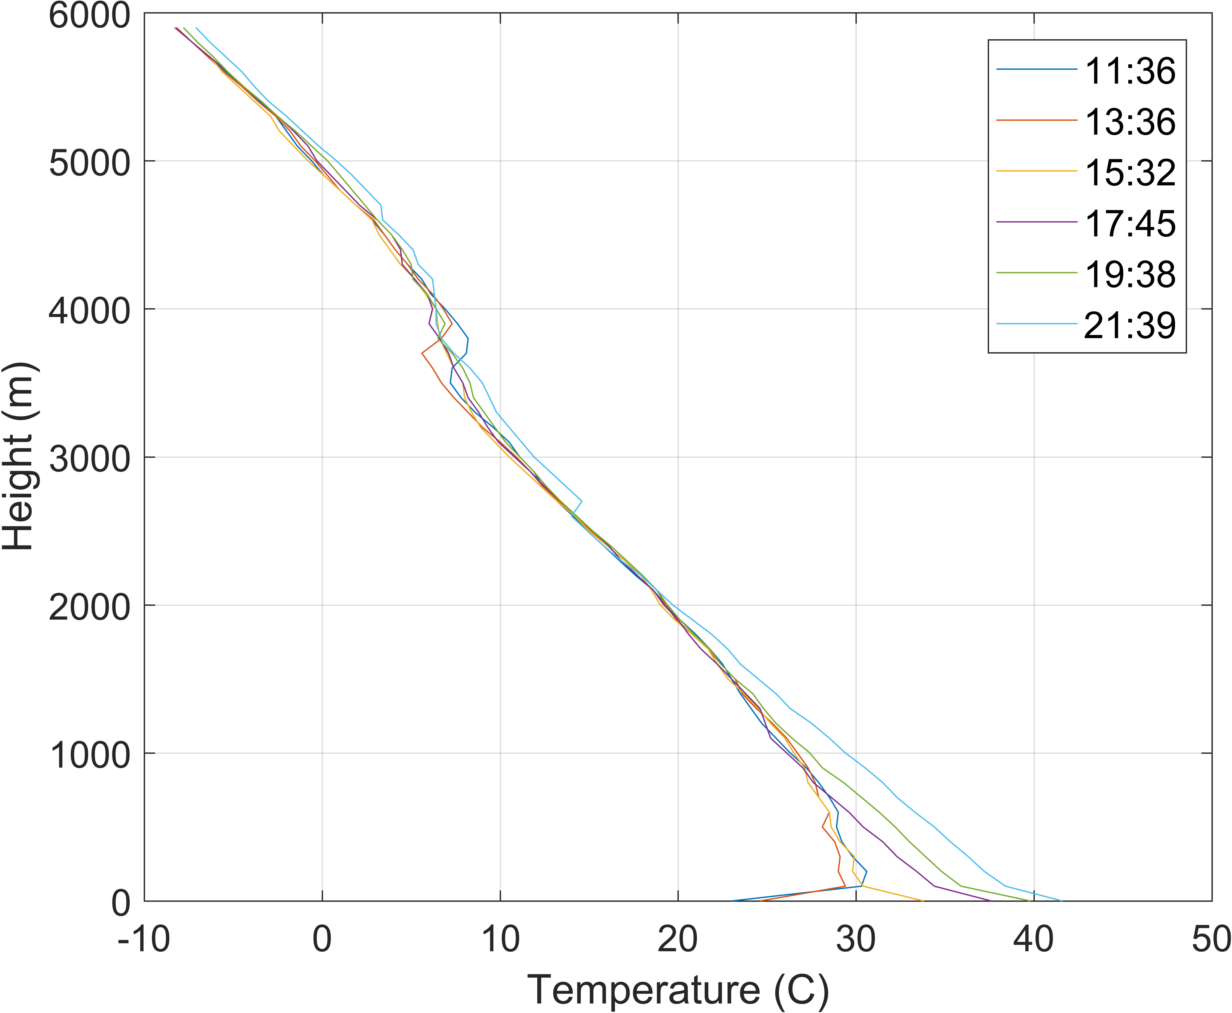
\includegraphics[width=\textwidth]{YumaTemp.png}
	\caption{Temperature profile over Yuma, AZ.}
	\label{fig:YumaT}
\end{figure}

\begin{figure}
	\centering
	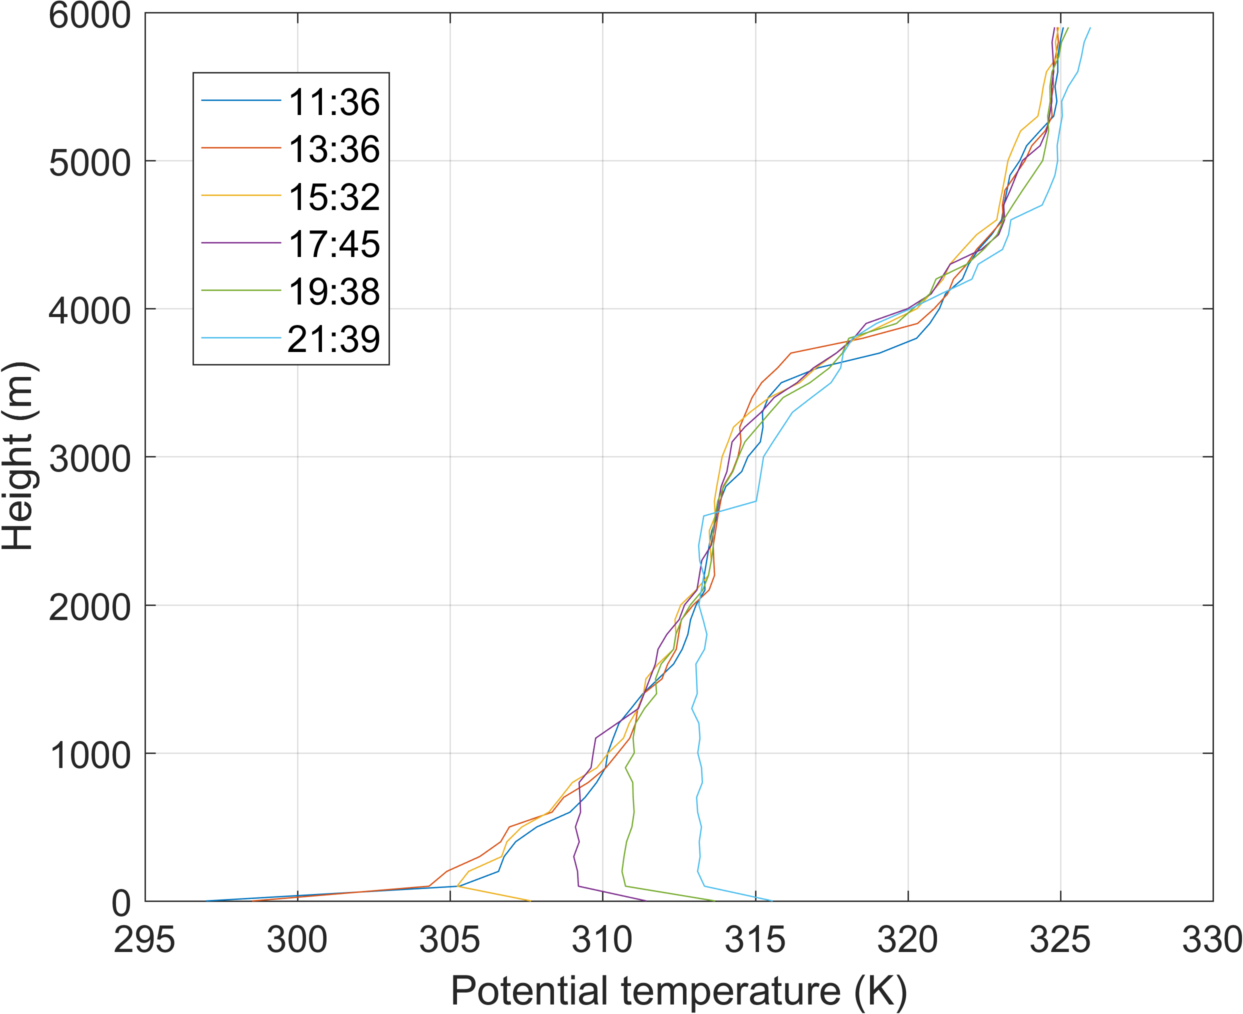
\includegraphics[width=\textwidth]{YumaPotentialTemp.png}
	\caption{Potential temperature $\displaystyle \theta(T) = T\left(\frac{p_0}{p}\right)^R/c_p$ profile over Yuma, AZ.}
	\label{fig:YumaPotentialT}
\end{figure}

We see the surface temperature drop during the day and stabilize a bit during the night.

\section{Moist convection}


%\begin{thebibliography}{9}
%\bibitem{AMSVirtualTemp}
%American Meteorological Society, cited 2012: Virtual temperature. Glossary of Meteorology. [Available online at \url{http://glossary.ametsoc.org/wiki/Virtual_temperature}]
%
%\bibitem{Wallace}
%Wallace, John M. and Peter V. Hobbs. \textit{Atmospheric Science; An Introductory Survey}. Elsevier. Second Edition, 2006. Chapter 1.
%\end{thebibliography}

\end{document}